\documentclass[11pt]{article}

% "review" gives line numbers and page numbers, as in the course reference.
% The \acl@anonymizefalse line below keeps author names visible.
% Keep "review" while the team reviews the draft (the rubric review cites line numbers).
% For the submitted copy without line numbers, change "review" to "preprint".
\usepackage[review]{acl}
\makeatletter\acl@anonymizefalse\makeatother

\usepackage{times}
\usepackage{latexsym}
\usepackage[T1]{fontenc}
\usepackage[utf8]{inputenc}
\usepackage{microtype}
\usepackage{inconsolata}
\usepackage{graphicx}
\usepackage{booktabs}
\usepackage{array}
\usepackage{xcolor}
\usepackage{amsmath,amssymb}
\usepackage{enumitem}
\usepackage{tikz}
\usetikzlibrary{positioning, arrows.meta}

% ----------------------------------------------------------------------------
% Markers for open items. The submitted report has none of them left
% (rubric gate 6). To list them: grep -n '\\todo\|\\tbd\|\\placeholderfig' sections/*.tex
% ----------------------------------------------------------------------------
% Red, bracketed marker for anything still to be written or measured.
\newcommand{\todo}[1]{\textcolor{red}{[TODO: #1]}}
% A table cell whose number is not measured yet.
\newcommand{\tbd}{\textcolor{red}{?}}
% A framed box that holds the place of a figure: \placeholderfig{width}{height}{what goes here}
\newcommand{\placeholderfig}[3]{\fbox{\parbox[c][#2][c]{#1}{\centering\todo{#3}}}}

% The teaser figure below the authors needs room, so shrink the default title box.
\setlength\titlebox{3.3cm}

\title{Knowing When Not to Trust Depth:\\
A Learned Per-Pixel Confidence Head for Monocular Depth\\
in Adverse Driving Conditions}

\author{Nathan Aday, Alejandro Arteaga, Nathan Bao, Katherine Qiao, Varad Jaideep Tawde}

\begin{document}

% Teaser. It still shows one cache entry (the inputs and the label). For the final
% report, replace it with a result: one night or rain image, its lidar AbsRel, and the
% head's confidence map side by side (src/evals/plot.py, qualitative_figure). The cache
% entry figure then moves to Appendix C.
\makeatletter
\g@addto@macro\@maketitle{%
  \begin{center}
    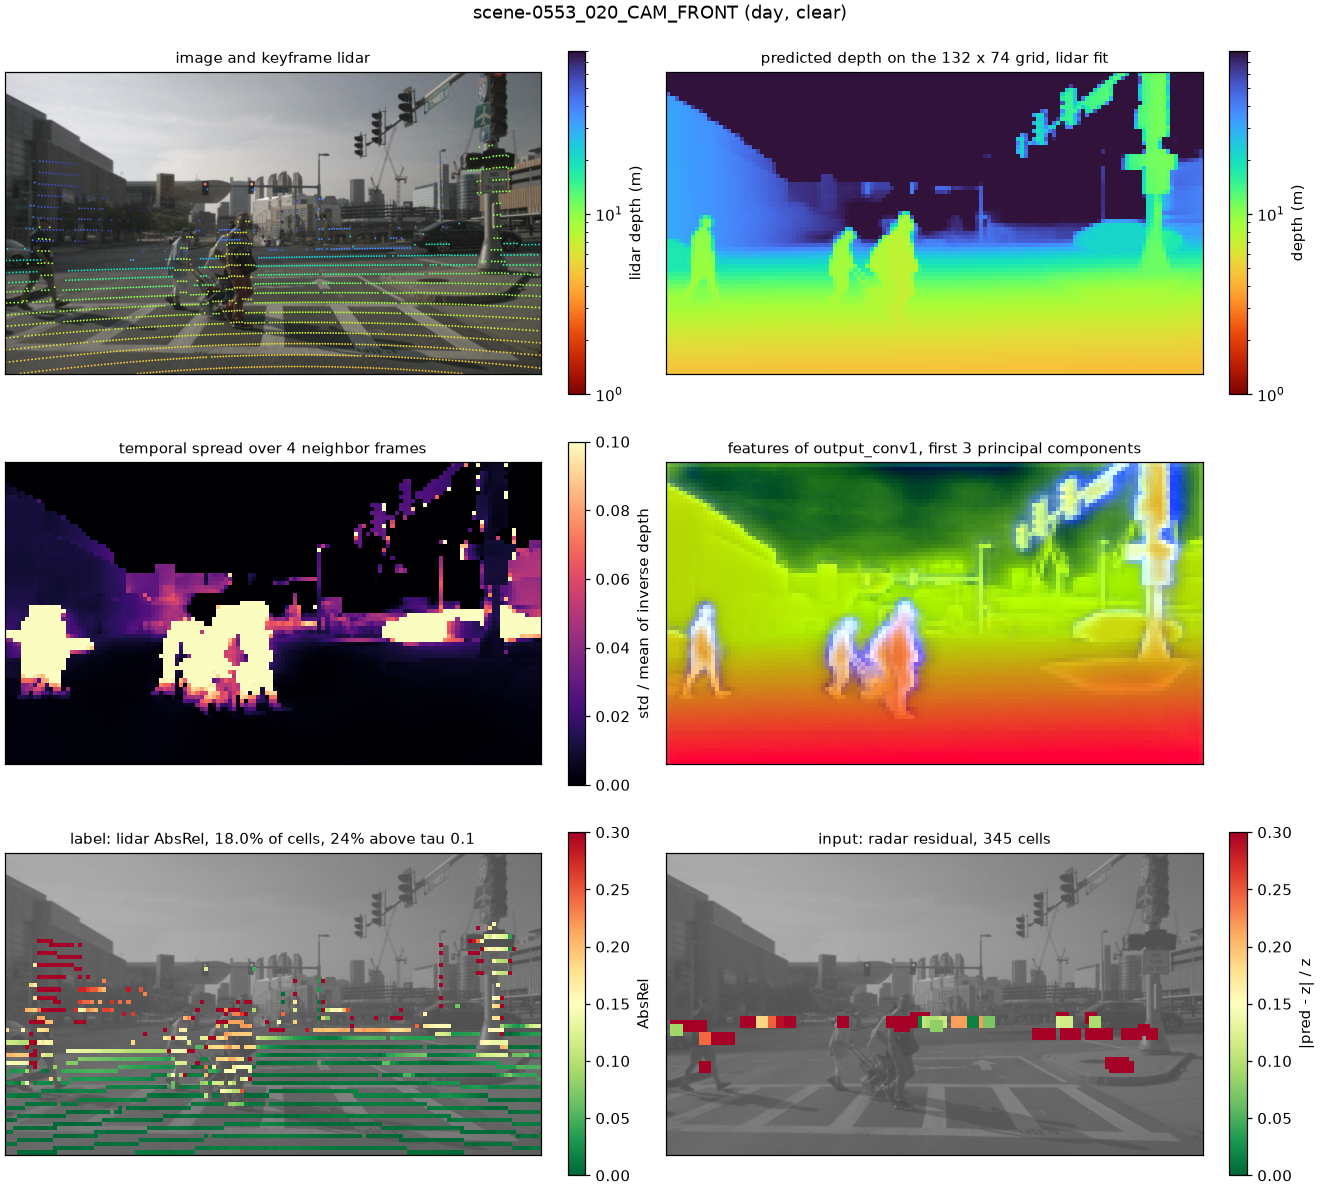
\includegraphics[width=0.46\textwidth]{figures/cache-entry-preview.png}
    \captionof{figure}{\todo{Replace with image / lidar AbsRel / confidence of one adverse-condition frame.} One cache entry (nuScenes scene-0553, CAM\_FRONT, day). Top: the image with projected keyframe lidar, and the Depth Anything V2 prediction after the lidar fit. Middle: the temporal spread input and the first three principal components of the 64 decoder features. Bottom: the lidar AbsRel label on the grid, and the radar residual input. The head reads the middle-left temporal spread and the three right-hand quantities, with a radar validity mask that is not shown, and must predict the bottom-left map. Two panels differ from what the head sees. The top-right depth is in meters after the lidar fit, while the head reads the disparity divided by its image mean, and the bottom-left AbsRel is drawn before thresholding at $\tau = 0.10$.}
    \label{fig:teaser}
  \end{center}
  \vskip 0.05in}
\makeatother

\maketitle

% ----------------------------------------------------------------------------
% Body: at most 8 pages (rubric gate 8). Each section lives in its own file
% under sections/. The page budget of each section is in its header comment
% and in ../README.md.
% ----------------------------------------------------------------------------
% !TEX root = ../main.tex
% ============================================================================
% Written last, once the numbers of Section 5 are final.
%
% Shape (150 to 200 words): problem (1 sentence), approach (1 to 2), setup (1),
% headline numbers (2 to 3), what they mean (1).
% Rubric gate 1: every claim here points to a number, table, or figure in the body.
% ============================================================================
\begin{abstract}
Monocular depth models such as Depth Anything V2 return a depth value for every pixel and no indication of which values to trust. We train a small convolutional head that reads the frozen depth model's decoder features, its predicted depth, the temporal spread of depth across neighboring frames, and two radar channels, and outputs per cell the probability that the depth error exceeds a fixed threshold. Labels come from lidar projected into the camera image, so no hand annotation is needed. On nuScenes, we train 18 heads that differ in their inputs, radar settings, label threshold, and training data, on a cache of all 204,894 trainval camera images.\footnote{\raggedright Code: \url{https://github.com/kgqiao/monocular-depth-confidence-estimation}} \todo{Two or three sentences with the headline numbers once the scores are final. (1) AUSE and AURG of the best head that needs no lidar at inference, against flip disagreement and the oracle. (2) The gap between day, rain, and night. (3) What the input ablation shows: decoder features, temporal spread, radar. Then one closing sentence on what this means for a consumer of the depth.}
\end{abstract}

% !TEX root = ../main.tex
% ============================================================================
% Owner: Arteaga
% ============================================================================
\section{Introduction}

Depth Anything and similar models supply depth to systems that have no depth sensor. They are used in driving, robotics, augmented reality, and 3D reconstruction, usually as a drop-in component. Every pixel gets a depth value and no measure of reliability: an estimate that is wrong by thirty percent looks exactly like one that is right. The cost of that silence is highest in the conditions where camera depth is least reliable: night, rain on the lens, spray, and low sun. A confidence map lets a downstream consumer weight the depth, discard it, or fall back to another sensor.

This project trains a model to predict that error without touching the depth model. A small convolutional head reads the frozen model's internal features along with its predicted depth, the temporal spread of depth across neighboring frames, a radar residual, and a radar validity mask. It outputs, per cell of a $132 \times 74$ grid, the probability that the depth there is wrong by more than a threshold; the confidence is one minus that probability. Lidar projected into the image gives the true error at the cells that receive a return, so the head learns from scattered labels and produces a dense map at inference. Training needs lidar. The design goal is that inference does not, while radar, which a production car does carry, is present in both. So far the heads meet that goal only in part. The temporal spread is computed with a lidar fit of the depth scale, so a head that reads it still depends on lidar; a head that leaves it out, such as the one that reads the decoder features alone, does not (Section~\ref{sec:runs}).
   % 1  Introduction               0.9 page
% !TEX root = ../main.tex
% ============================================================================
% Budget: 0.8 page (the midterm version ran about 1.5 pages, so this needs a trim).
% Each paper gets what it does and the one fact we use; the contrast with our
% work is stated once, in the closer.
%
% Carried over from the midterm literature review. Still to do (checklist B5):
% add Sudhakar et al. 2022 (uncertainty from motion) and Singh et al. 2023
% (radar-camera depth), each with a bib entry checked against arXiv.
%
% Papers in Docs/Papers/ are named by arXiv id, one PDF per bib entry.
% Every bib entry was checked against arXiv on 2026-11-06.
% ============================================================================
\section{Related Work}
\label{sec:related}

\todo{Trim this section to 0.8 page, and add Sudhakar et al.\ 2022 and Singh et al.\ 2023.}

\paragraph{Monocular depth foundation models.}
Our backbone belongs to a family of models trained to predict relative depth from a single image across many datasets. MiDaS \citep{ranftl2020midas} trains on datasets with incompatible annotations by using a loss that aligns prediction and ground truth in scale and shift before comparing them. The network therefore predicts inverse depth only up to those two unknowns, which are fitted per image by least squares before any error is measured. Our per-image fits against lidar and radar are the same alignment, done with sparse sensor returns. DPT \citep{ranftl2021dpt} replaces the convolutional encoder with a vision transformer whose tokens are reassembled into feature maps at four resolutions and merged by a convolutional decoder, followed by a short convolutional head. Depth Anything \citep{yang2024depthanything} and Depth Anything V2 \citep{yang2024depthanythingv2} pair a DINOv2 encoder with this decoder and scale the training data by pseudo-labeling about 62M unlabeled images with a teacher model. The first convolution of the head, named \texttt{output\_conv1} in the V2 code, gives the 64-channel map for ViT-B that our head reads. The released models output affine-invariant inverse depth and no per-pixel confidence; we use the relative ViT-B checkpoint frozen (deviation D1 in Table~\ref{tab:deviations}).

\paragraph{Uncertainty and confidence for monocular depth.}
Most work on uncertainty for depth changes the depth model. \citet{kendall2017uncertainties} separate aleatoric uncertainty, the noise inherent in the observations, from epistemic uncertainty, which lies in the model, and estimate the first with a variance output learned through the loss and the second with Monte Carlo dropout \citep{gal2016dropout}, which runs the network several times with resampled dropout masks. Deep ensembles \citep{lakshminarayanan2017ensembles} train several networks from different initializations and combine their predictions. All three are trained with the depth network or need several copies of it, which a single frozen checkpoint rules out. Our proposal listed MC dropout as a baseline; we drop it because every dropout rate in the Depth Anything V2 encoder is zero and the decoder has none, so repeated passes are identical (Appendix~\ref{app:deviations}).

\citet{poggi2020uncertainty} compare eleven ways of estimating per-pixel uncertainty for a self-supervised depth network (Monodepth2 on KITTI) and supply our evaluation protocol. Pixels are removed in order of decreasing uncertainty and the error of the remainder is plotted. AUSE, introduced for optical flow by \citet{ilg2018uncertainty}, is the area between that sparsification curve and the oracle curve that removes pixels by true error (lower is better); AURG is the area between the flat curve of a random ordering and the model's curve (higher is better). The paper gives both in words, so how the areas are computed over our labeled grid cells is our own choice. Its ``Post'' method, the difference between the depth of an image and the flipped-back depth of its mirror image, needs no retraining, and our flip-disagreement baseline is adapted from it. The paper also notes that a classifier trained on the prediction error, which is what our head is, is common in stereo and optical flow but needs ground-truth depth; our lidar supplies it.

\citet{hornauer2022gradient} estimate uncertainty for a trained depth network without changing its weights and without any training. The difference between the depth maps of an image and its horizontal flip is used as a loss, and the gradient of that loss at one decoder layer, pooled over channels, is the uncertainty map. On Monodepth2 it ranks errors better than the plain flip difference, at the cost of a backward pass per image. It is among the nearest prior work to ours in leaving the depth model untouched and reading its decoder, but it uses no ground truth. We leave it out of our baselines, because it needs a backward pass per image and our cache stores the decoder activations without the graph a gradient needs.

Two methods train a second network on ground truth, as we do. ConfidNet \citep{corbiere2019confidnet} learns the confidence of a trained classifier: an auxiliary network reads the classifier's features and is trained to predict the probability the classifier gives to the true class. SLURP \citep{yu2021slurp} carries the idea to regression, monocular depth among its tasks, with a side network that reads the output and the intermediate features of the main model. Our head follows this pattern in a different setting: a frozen foundation model, sparse lidar labels, and radar and temporal inputs.

\paragraph{Radar-camera fusion.}
Recent work fuses radar with images to improve depth or 3D perception; we instead give radar to the head as evidence of where the frozen depth disagrees with an independent range measurement. \citet{lin2020radardepth} predict dense depth on nuScenes from an image and sparse projected radar, and list what makes radar harder to use than lidar: far fewer points, a limited vertical field of view, noise from multipath reflections, and disagreement with lidar even for clean returns. Their network discards radar points that disagree with a first depth estimate. Our radar residual is the same comparison, passed to the head as an input instead of being thresholded, and its noise in our data (Section~\ref{sec:data}) agrees with their account. HyDRa \citep{wolters2025hydra} and LiCROcc \citep{ma2024licrocc} bring radar into networks for 3D detection and occupancy, the first by fusing radar features before the depth network and the second by distilling a lidar-camera teacher into a radar-camera student; Occ3D \citep{tian2023occ3d} is the occupancy benchmark of the stretch goal in our proposal, now left as future work (Section~\ref{sec:conclusion}). BEVCar \citep{schramm2024bevcar} fuses cameras and radar for bird's-eye-view segmentation and releases a division of the nuScenes validation set into day, rain, and night groups of 4,449, 968, and 602 samples, which we use for our per-condition results.

\paragraph{Adverse-condition driving datasets.}
nuScenes \citep{caesar2020nuscenes}, the dataset we train and evaluate on, provides 1,000 driving scenes of 20 seconds with six cameras, a 32-beam lidar, and five radars, with rain and night at 19.4\% and 11.6\% of keyframes. Camera exposure is triggered as the lidar sweeps across each camera's field of view, which lets us project lidar into the image as labels, and the radar sweeps between keyframes are released, which our radar residual accumulates. md4all \citep{gasperini2023md4all} makes a depth network robust at night and in rain by training on day images translated to those conditions; evaluated per condition against lidar on nuScenes, its self-supervised baselines show depth error roughly doubling from day to night, the direction we see in our own cache (Section~\ref{sec:data}).
% Access terms ("by request") are not in the paper; cite the project page before stating them here.
Seeing Through Fog \citep{bijelic2020seeing}, STF below, has the fog and snow that nuScenes lacks, with lidar and radar, and was our candidate for a second evaluation, now left as future work (Section~\ref{sec:conclusion}), though adverse frames are a small part of its labeled set and lidar's perceivable distance falls to about 25\,m in fog.
% The radar added in the 2025 ZOD release is not in this paper; cite the release before mentioning it.
The Zenseact Open Dataset \citep{alibeigi2023zod}, ZOD below, offers 20-second camera and lidar sequences but, as described in the paper, no radar, so it ranks behind STF as a second dataset.

\paragraph{Where this work sits.}
The depth foundation models return relative depth with no indication of reliability; we take one as given and add that indication. The uncertainty literature mostly builds the estimate into the depth network or samples it, which a frozen public checkpoint does not allow, and most of the post-hoc methods that remain use no ground truth. Like ConfidNet and SLURP, we train a small second network on error labels; ours come from lidar, and we evaluate the head with that literature's sparsification measures. Radar-camera work uses radar to improve the prediction itself; we use it to predict where the depth is wrong. Whether the frozen decoder features carry enough information to predict the model's own error, and how much radar and the temporal spread add, are the questions the experiments answer.
   % 2  Related Work               0.8 page
% !TEX root = ../main.tex
% ============================================================================
% Budget: 1.5 pages, with Figure 2 (pipeline) and Table 1 (inputs).
%
% This section says what the method IS, in the present tense, so that a reader
% could build it again. It holds no results, no cluster detail, and no history
% of how the team got here: results go to Section 5, the cache and the cluster
% to Appendix C, the differences from the proposal to Appendix A.
%
% The prose of 3.2 to 3.4 is carried over from the midterm report (Method as
% Implemented). The equations of 3.1 are new and were written from
% confhead/src/confhead/labels.py, geometry.py (Fit, fit_scale_shift) and
% head.py (masked_bce); the owners should check them against the code.
% ============================================================================
\section{Method}
\label{sec:method}

Figure~\ref{fig:pipeline} shows the pipeline from the raw data to the loss. Only the head is trained; everything to its left is computed once per image and cached.

\begin{figure*}[t]
  \centering
  \resizebox{\textwidth}{!}{% Pipeline of the confidence head, condensed from Docs/Wiki/Models/run1/run1.canvas.
% Needs tikz with the libraries positioning and arrows.meta (loaded in main.tex).
\begin{tikzpicture}[
    font=\scriptsize,
    box/.style={draw=black!45, rounded corners=1.5pt, align=center, text width=2.55cm,
                minimum height=0.82cm, inner sep=2pt},
    raw/.style={box, fill=orange!18},
    calc/.style={box, fill=violet!12},
    cache/.style={box, fill=cyan!15},
    chan/.style={box, fill=green!18},
    lab/.style={box, fill=yellow!30},
    head/.style={box, fill=black!6},
    arr/.style={-{Stealth[length=1.6mm]}, draw=black!60, line width=0.4pt},
    colhead/.style={font=\scriptsize\bfseries, align=center, text width=2.9cm},
  ]
  % Columns: x = 0, 3.25, 6.5, 9.75, 13. Rows: y = 0, -1.05, -2.1, -3.15, -4.45.
  \node[colhead] at (0, 0.85)     {nuScenes data};
  \node[colhead] at (3.25, 0.85)  {Cache build\\(once per image)};
  \node[colhead] at (6.5, 0.85)   {Cache entry};
  \node[colhead] at (9.75, 0.85)  {Head input\\(set per run)};
  \node[colhead] at (13, 0.85)    {Trained};

  % Raw data
  \node[raw] (rimg) at (0, -0.525) {Camera keyframe\\$1600 \times 900$, 6 cameras};
  \node[raw] (rnbr) at (0, -2.1)   {Neighbor frames\\$\pm 1, \pm 2$ at 12\,Hz};
  \node[raw] (rrad) at (0, -3.15)  {Radar points\\5 sweeps, no elevation};
  \node[raw] (rlid) at (0, -4.45)  {Lidar points\\never an input};

  % Cache build
  \node[calc, minimum height=1.87cm] (da2) at (3.25, -0.525) {Frozen Depth\\Anything V2 ViT-B\\at $924 \times 518$};
  \node[calc] (btmp) at (3.25, -2.1)  {4 extra passes; follow each cell's 3D point};
  \node[calc] (brad) at (3.25, -3.15) {Project to camera;\\radar fit};
  \node[calc] (blid) at (3.25, -4.45) {Project to camera;\\lidar fit};

  % Cache entry
  \node[cache] (cfeat) at (6.5, 0)     {Decoder features\\\texttt{output\_conv1}, fp16};
  \node[cache] (cdisp) at (6.5, -1.05) {Disparity grid};
  \node[cache] (ctmp)  at (6.5, -2.1)  {Temporal spread};
  \node[cache] (crad)  at (6.5, -3.15) {Radar points, fit\\(scale, shift)};
  \node[cache] (clid)  at (6.5, -4.45) {Lidar points, fit\\(scale, shift)};

  % Head input and labels
  \node[chan] (ifeat) at (9.75, 0)     {Features (64)};
  \node[chan] (idep)  at (9.75, -1.05) {Depth (1)\\disparity / image mean};
  \node[chan] (itmp)  at (9.75, -2.1)  {Temporal spread (1)};
  \node[chan] (irad)  at (9.75, -3.15) {Radar residual and validity (2)};
  \node[lab]  (ilab)  at (9.75, -4.45) {Target $\mathbf{1}[\mathrm{AbsRel} > \tau]$ and label mask};

  % Head and loss
  \node[head, minimum height=3.97cm] (head) at (13, -1.575)
    {\textbf{Confidence head}\\[2pt]standardize channels\\$3 \times 3$ conv, 64\\$3 \times 3$ conv, 64\\$3 \times 3$ conv, 32\\$1 \times 1$ conv\\[2pt]$p_\mathrm{error}$ per grid cell};
  \node[lab] (loss) at (13, -4.45) {Masked BCE on labeled cells};

  % Edges
  \draw[arr] (rimg) -- (da2);
  \draw[arr] (da2.east |- cfeat) -- (cfeat);
  \draw[arr] (da2.east |- cdisp) -- (cdisp);
  \draw[arr] (rnbr) -- (btmp);
  \draw[arr] (rrad) -- (brad);
  \draw[arr] (rlid) -- (blid);
  \draw[arr] (btmp) -- (ctmp);
  \draw[arr] (brad) -- (crad);
  \draw[arr] (blid) -- (clid);
  \draw[arr, dashed] (blid.west) -- ++(-0.22, 0) |- (btmp.west);
  \draw[arr] (cfeat) -- (ifeat);
  \draw[arr] (cdisp) -- (idep);
  \draw[arr] (ctmp) -- (itmp);
  \draw[arr] (crad) -- (irad);
  \draw[arr] (clid) -- (ilab);
  \draw[arr] (ifeat) -- (ifeat -| head.west);
  \draw[arr] (idep) -- (idep -| head.west);
  \draw[arr] (itmp) -- (itmp -| head.west);
  \draw[arr] (irad) -- (irad -| head.west);
  \draw[arr] (ilab) -- (loss);
  \draw[arr] (head) -- node[right, font=\tiny] {logits} (loss);
\end{tikzpicture}
}
  \caption{The pipeline. Orange: raw nuScenes data. Violet: a computation done once per image when the cache is built. Cyan: an array stored in the cache. Green: an input group of the head, which a run can switch off (Table~\ref{tab:input-ablation}). Yellow: the lidar labels and the loss. The dashed arrow marks that the temporal spread uses the lidar fit to lift each cell to a 3D point.}
  \label{fig:pipeline}
\end{figure*}

% ----------------------------------------------------------------------------
\subsection{Problem Formulation}
\label{sec:formulation}
% New for the final report (checklist B5: numbered equations).
% \todo for the owners: check each equation against the code named above.

The depth model returns a disparity map $q$ that is inverse depth up to an unknown scale and shift. For an image with lidar returns $i = 1, \dots, N$ at depths $z_i$, let $q_i$ be the disparity sampled at the pixel of return $i$. We fit the two unknowns per image by least squares against inverse depth,
\begin{equation}
  (s, t) = \operatorname*{arg\,min}_{s,\,t} \sum_{i=1}^{N} \Bigl( s\,q_i + t - \frac{1}{z_i} \Bigr)^{2},
  \label{eq:fit}
\end{equation}
and call the fit failed when $s \le 0$ or the returns are too few. The predicted depth at a return clips the fitted inverse depth to the range of the labels before inverting it,
\begin{equation}
  \hat d_i = \Bigl[ \operatorname{clip}\bigl( s\,q_i + t,\ 1/z_{\max},\ 1/z_{\min} \bigr) \Bigr]^{-1},
  \label{eq:depth}
\end{equation}
with $z_{\min} = 1$\,m and $z_{\max} = 80$\,m. The error of the depth at a return is its absolute relative error,
\begin{equation}
  e_i = \frac{|\hat d_i - z_i|}{z_i}.
  \label{eq:absrel}
\end{equation}
Because of Eq.~\ref{eq:fit}, $e_i$ is the error under the best scale and shift of that image: it measures the shape of the depth, and a frame whose overall scale is off still counts as correct.

Let $c$ index the cells of the output grid, let $M$ be the set of cells that receive at least one return, and let $e_c$ be the error of the nearest return in cell $c \in M$. The label is
\begin{equation}
  y_c = \mathbf{1}\,[\, e_c > \tau \,], \qquad \tau = 0.10 .
  \label{eq:label}
\end{equation}
The head $f_\theta$ maps the input $x$ (Section~\ref{sec:inputs}) to one logit per cell, and
\begin{equation}
  p_c = \sigma\bigl( f_\theta(x)_c \bigr)
  \label{eq:perror}
\end{equation}
is its estimate of the probability that $y_c = 1$. The confidence of cell $c$ is $1 - p_c$. The head is trained on the cells in $M$ and predicts for every cell.

\todo{Check Eqs.~\ref{eq:fit} to \ref{eq:perror} against \texttt{labels.py}, \texttt{geometry.py}, and \texttt{head.py}; state the minimum number of returns for a fit.}

% ----------------------------------------------------------------------------
\subsection{Frozen Backbone and Head Inputs}
\label{sec:inputs}

\paragraph{Backbone.} The backbone is the stock relative Depth Anything V2 ViT-B checkpoint \citep{yang2024depthanythingv2}, frozen and run once per image at $924 \times 518$. Its output is disparity with unknown scale and shift, so each cached entry carries two per-image fits of the form of Eq.~\ref{eq:fit}: one against the keyframe lidar, used for the labels and the temporal channel, and one against the radar points, used for the radar residual.

\paragraph{Inputs.} Everything lives on a $132 \times 74$ grid, the ViT patch grid times two, where one cell covers about $12 \times 12$ pixels of the $1600 \times 900$ camera image. We use times two to fit the storage (about 290\,GB, against 1.1\,TB at times four). The head input has 68 channels (Table~\ref{tab:inputs}), each standardized by its training-set mean and standard deviation. Channel groups can be switched off at load time, which is how the ablation runs of Section~\ref{sec:input-ablation} are made.

\begin{table}[t]
  \centering
  \small
  \setlength{\tabcolsep}{4pt}
  \begin{tabular}{@{}l l p{3.2cm}@{}}
    \toprule
    \textbf{Ch.} & \textbf{Input} & \textbf{How it is made} \\
    \midrule
    0--63 & Decoder features & \texttt{output\_conv1} tap, 64 channels, area-averaged to the grid \\
    64 & Norm.\ disparity & Disparity divided by its image mean; no fit \\
    65 & Temporal spread & Std divided by mean ($\sigma/\mu$) of inverse depth over the keyframe and its neighbors at $\pm1, \pm2$ (12\,Hz; up to 5 frames), ego-motion compensated \\
    66 & Radar residual & $|\hat d - z| / z$ under the radar fit, 5 sweeps, radius 1 cell \\
    67 & Radar validity & 1 where the residual holds a measurement \\
    \bottomrule
  \end{tabular}
  \caption{The 68 input channels of the confidence head. Channel 64 is called the depth channel in the rest of the report. In channel 66, $\hat d$ is the depth that the radar fit gives the model's disparity at a radar point, $z$ is the range of that point, and the nearest point wins a cell where two footprints overlap.}
  \label{tab:inputs}
\end{table}

% ----------------------------------------------------------------------------
\subsection{Lidar-Derived Labels}
\label{sec:labels}

For each lidar return within 1--80\,m, the absolute relative error (AbsRel, Eq.~\ref{eq:absrel}) of the fitted prediction at that pixel is placed in its grid cell; the nearest point wins a cell. Here the prediction is the model disparity sampled at the return's own pixel and passed through the lidar fit (Eq.~\ref{eq:depth}). The target is Eq.~\ref{eq:label}, and a mask marks the labeled cells. About 25\% of cells on the $132 \times 74$ grid carry a label, about 2,450 per image. The lidar returns behind them, about 3,600 per image, cover 0.25\% of pixels. \todo{Refresh the three counts on the complete cache, and say how the label masks were settled: the ego body in CAM\_BACK (D8), bleed-through returns (D9), and images with no lidar fit (D13). These change the labels, so they must be settled before the final scoring (checklist B1).}

% ----------------------------------------------------------------------------
\subsection{Confidence Head and Loss}
\label{sec:head}

The head is three $3 \times 3$ convolutions (stride 1 and padding 1, so the grid size is kept) with ReLU and widths 64, 64, 32, then a $1 \times 1$ convolution to one logit per cell. With all 68 inputs it has 94,657 weights, and its receptive field is $7 \times 7$ cells. The loss is binary cross-entropy (BCE) over the labeled cells only, with positives weighted by the negative-to-positive ratio $w_+$ of the training labels:
\begin{equation}
  \mathcal{L} = -\frac{1}{|M|} \sum_{c \in M} \Bigl[ w_+\, y_c \log p_c + (1 - y_c) \log (1 - p_c) \Bigr].
  \label{eq:loss}
\end{equation}
This weight raises every logit by $\ln w_+$ (\todo{Refresh; 0.506 for $w_+ = 1.658$ on the partial cache; give the value of the complete cache}). The ranking metrics are unaffected, but the calibration shifts, so we report the expected calibration error (ECE) after subtracting it (Section~\ref{sec:protocol}).

% ----------------------------------------------------------------------------
\subsection{Sensors Needed at Inference}
\label{sec:sensors}
% New subsection. It answers the critical item of the midterm review (A1, A2,
% B1 "lidar in the inputs") in one place, so that the results can refer to it.
% Rubric gate 4 checks this subsection.

Training needs lidar for the labels. Whether inference needs it depends on the inputs a head reads. The decoder features and the normalized disparity need no fit. The radar residual uses the radar fit, which a production car can compute. The temporal spread lifts each cell to a 3D point with the lidar fit, so every head that reads it uses lidar at inference and is an upper bound for a deployed system. Two heads are therefore free of lidar: \texttt{m1-features-only}, which reads the decoder features alone and needs no sensor fit at all, and \texttt{m1-no-temporal}. Table~\ref{tab:main} marks each method accordingly.

\todo{State the team's decision on checklist item B1. Either (a) the temporal channel was rebuilt without lidar, or (b) it was kept and the lidar-free heads are presented as the deployable models, with the 68-channel head and \texttt{m2-radar-lidar-fit} as upper bounds. This paragraph assumes (b).}
         % 3  Method                     1.5 pages
% !TEX root = ../main.tex
% ============================================================================
% Budget: 1.2 pages, with Table 2 (label counts per condition).
%
% This section fixes everything a reader needs in order to trust Section 5:
% the data, how the heads were trained, what they are compared with, and how
% each number is computed. It is written before the results are read, and it
% does not change afterwards (rubric: experimental design and rigor).
%
% Carried over from the midterm report: the training settings, the BEVCar
% split, the flip baseline, and the metric definitions. The detail of the
% cache and of the cluster is in Appendix C.
% ============================================================================
\section{Experimental Setup}
\label{sec:setup}

% ----------------------------------------------------------------------------
\subsection{Dataset, Cache, and Condition Splits}
\label{sec:data}

We train and evaluate on nuScenes v1.0 trainval \citep{caesar2020nuscenes} with its official split of 700 training and 150 validation scenes. The backbone runs once per image, and its outputs are stored in a cache of head inputs that holds all 204,894 trainval camera images, of which 36,114 are validation images. Labels and radar channels are computed when an entry loads, so $\tau$, the radar radius, and the choice of fit are settings of a run and need no rebuild (Appendix~\ref{app:cache}).

\paragraph{Condition groups.} We report every result for day, rain, and night with the division of the validation scenes released with BEVCar \citep{schramm2024bevcar}: 111 day, 24 rain, and 15 night scenes, which together are the 150 validation scenes. Three scenes are tagged both night and rain; the division places them in night. Table~\ref{tab:labelcounts} gives the images and the lidar labels of each group, so that a lack of labels in one condition is visible next to its scores.

\begin{table}[t]
  \centering
  \small
  \setlength{\tabcolsep}{4pt}
  \begin{tabular}{@{}l r r r r@{}}
    \toprule
    & \textbf{Scenes} & \textbf{Images} & \textbf{Labels / image} & \textbf{Wrong} \\
    \midrule
    Day   & 111 & \tbd & \tbd & \tbd\,\% \\
    Rain  &  24 & \tbd & \tbd & \tbd\,\% \\
    Night &  15 & \tbd & \tbd & \tbd\,\% \\
    \midrule
    All   & 150 & \tbd & \tbd & \tbd\,\% \\
    \bottomrule
  \end{tabular}
  \caption{The validation split by condition: scenes, scored images, labeled cells per image, and the share of labeled cells whose AbsRel exceeds $\tau = 0.10$. \todo{Fill from \texttt{label\_count\_table.py} on the complete cache. The committed \texttt{lidar\_pixels\_per\_condition.csv} counts 26,207 images, which is the partial cache; the complete cache has 36,114 validation images.}}
  \label{tab:labelcounts}
\end{table}

\paragraph{What the data says before any head is trained.} Night is harder than day: on the development cache the median per-image AbsRel is 0.052 by day and 0.079 at night. The radar residual is noisy and sparse: its median is about five times the lidar-measured depth error, and the radar validity channel marks 3.4\% of the grid cells. Appendix~\ref{app:cache} has the full statistics. \todo{Refresh these numbers on the complete cache; they are from the mini cache and the partial trainval cache.}

% ----------------------------------------------------------------------------
\subsection{Training}
\label{sec:training}

We train with AdamW at a learning rate of $10^{-3}$ and a weight decay of $10^{-4}$, on a cosine schedule, with batch size 8, for 8 epochs. The dev split is 10\% of the training scenes, and we compute the dev loss on a fixed random subset of 3,000 of its images. We keep the checkpoint with the lowest dev loss. \todo{Give the training time of one run and the GPU.}

\paragraph{Runs.} Every run changes one thing from this default, so each run answers one question. We trained 18 heads on the complete cache: the baseline with all inputs, its repeat, and a run without radar; seven runs that remove or isolate an input group or change the seed; four that change the radar settings; two that move $\tau$ to 0.05 and 0.2; and two that shorten the label range to 50\,m or train on a quarter of the data. Table~\ref{tab:runs} in Appendix~\ref{app:runs} lists them. The training seed also picks the dev scenes, so the seed run is compared with the others on the validation split only. \todo{Say whether the learning-rate, 16-epoch, and head-width runs (stage 4) and the final seeds (stage 5) were trained; if not, say so here in one sentence and in Section~\ref{sec:discussion}.}

% ----------------------------------------------------------------------------
\subsection{Compared Methods}
\label{sec:methods}
% One line per method: what the score is, and what it costs at inference.
% Rubric gate 2: every method in one table is scored on the same validation
% images and the same labeled cells. State the counts.

Every method gives each labeled cell a score, and the scores are compared on the same cells.

\begin{description}[leftmargin=1em, itemsep=1pt, topsep=2pt]
  \item[Random and oracle.] The two bounds of sparsification: a random order of the cells, and the order of the true error.
  \item[Flip disagreement.] The backbone runs on the image and on its mirror image, and the score of a pixel is the relative disagreement $|q - q'| / (|q| + |q'|)$ of the two disparity maps, averaged over each cell. It is adapted from the ``Post'' method of \citet{poggi2020uncertainty} and needs no training, at the cost of a second pass of the backbone.
  \item[Normalized disparity.] Channel 64 as a score, with the farthest cells removed first. It tests whether the head learns more than ``far is uncertain''. \todo{Not built yet (checklist B3).}
  \item[Temporal spread.] Channel 65 as a score, with no head: the simplest use of the temporal cue, and the score a trained head has to beat. \todo{Not built yet.}
  \item[Single-cue heads.] \texttt{m1-depth-only} and \texttt{m1-temporal-only}: a head trained on one channel.
  \item[Features-only head.] \texttt{m1-features-only}: the 64 decoder features and no other input. It needs no sensor at inference.
  \item[Full head.] \texttt{run-v1-radar}: all 68 inputs. It uses the lidar fit at inference through the temporal spread (Section~\ref{sec:sensors}).
\end{description}

We do not compare with Monte Carlo dropout, because every dropout rate in the Depth Anything V2 encoder is zero and the decoder has none, so repeated passes are identical; nor with the gradient method of \citet{hornauer2022gradient} (Section~\ref{sec:related}).

% ----------------------------------------------------------------------------
\subsection{Metrics and Protocol}
\label{sec:protocol}
% Rubric gate 3 and checklist B2. The three choices the midterm review asked us
% to write down are: (1) the error on the curve, (2) per image then averaged, or
% pooled, (3) whether a curve is normalized. The text below states what
% src/evals/metrics.py and examples/evaluate_head.py do today.

\paragraph{Sparsification.} Following \citet{poggi2020uncertainty}, the labeled cells of an image are removed in order of decreasing uncertainty $p_c$, and the mean AbsRel of the cells that remain is recorded at 50 removed fractions $\alpha$ from 0 to 0.99. This gives the curve $S(\alpha)$ of a method, the curve $S^{*}(\alpha)$ of the oracle that removes cells by their true error, and the flat curve $\bar e$ of a random order, which is the mean AbsRel of the image. Then
\begin{align}
  \mathrm{AUSE} &= \int_{0}^{0.99} \bigl( S(\alpha) - S^{*}(\alpha) \bigr)\, d\alpha, \label{eq:ause} \\
  \mathrm{AURG} &= \int_{0}^{0.99} \bigl( \bar e - S(\alpha) \bigr)\, d\alpha, \label{eq:aurg}
\end{align}
both by the trapezoid rule. AUSE is the distance from the oracle (lower is better, 0 is perfect) and AURG the gain over a random order (higher is better, 0 is random). The curves are in units of AbsRel and are not normalized. We compute both per image and average over the images of a group. \todo{Confirm ``per image, then averaged'' as the reported number, and say how images with a single labeled cell are handled.}

\paragraph{Classification and calibration.} The rejection AUROC is the area under the ROC curve for separating correct from wrong cells by confidence. The ECE uses 10 equal-width bins of confidence, and the Brier score is the mean squared difference between $p_c$ and $y_c$. We report the AUROC and the ECE pooled over all labeled cells of a group. \todo{Apply the logit correction of Section~\ref{sec:head} in \texttt{evaluate\_head.py} (subtract $\ln w_+$ before the sigmoid) and report the ECE before and after. Scores that are not probabilities, such as flip disagreement, get no ECE and no Brier score.}

\paragraph{Intervals.} \todo{Replace the image-level bootstrap of \texttt{build\_results\_table.py} with a paired bootstrap over scenes (checklist B2): resample the 150 validation scenes with replacement, keep the images of a scene together, $B = 1{,}000$, and report the 95\% interval of each score and of the difference between two methods. Frames of one scene are correlated, so an interval over images is too narrow.}

\paragraph{Evaluation set.} \todo{State the number of validation images and labeled cells that every method is scored on, and the number skipped for having no label. The flip baseline was scored on 26,207 images and the first head on 35,927; they must be scored on the same images before they share a table.}
          % 4  Experimental Setup         1.2 pages
% !TEX root = ../main.tex
% ============================================================================
% Budget: 2.3 pages. The page holds two full-width tables and two or three
% figures at most; anything more goes to Appendix D.
%
% HOW TO WRITE A SUBSECTION HERE
%   1. Start with the finding in one bold sentence, as the midterm results did.
%   2. Give the numbers that support it and point to the table or figure.
%   3. Say what limits the finding (scene count, interval, what was not run).
% Each subsection below has a comment with what it must show and where the
% numbers come from. Replace every \tbd and \todo; delete the comment last.
%
% WHERE THE NUMBERS COME FROM
%   per-image scores of a head   confhead/examples/evaluate_head.py  (CARC: carc-eval.sbatch)
%   flip baseline                confhead/examples/run_flip_baseline.py
%   tables with intervals        confhead/examples/build_results_table.py
%   figures                      confhead/src/evals/plot.py  -> ../figures-src/
%
% BEFORE ANY NUMBER GOES IN (rubric gates 2 and 3)
%   - All methods of a table are scored on the same validation images and cells.
%   - Intervals come from the paired bootstrap over scenes (Section 4.4).
%   - The label masks D8, D9, D13 are settled (Section 3.3).
% ============================================================================
\section{Results}
\label{sec:results}

% ----------------------------------------------------------------------------
\subsection{Main Comparison}
\label{sec:main}
% MUST SHOW: the head against every score that needs no training, and against
% the two bounds, on all validation images. One row per method of Section 4.3.
% The reader should see at a glance (a) how far the best head is from the
% oracle, (b) how much it gains over flip disagreement, and (c) what the
% lidar-free head loses against the full head.
% Negative results stay in the table (rubric gate 5): if a simple score matches
% a head, the row says so.

\todo{One bold sentence with the main finding, then the numbers of Table~\ref{tab:main} and the reading of Figure~\ref{fig:sparsification}.}

\begin{table*}[t]
  \centering
  \small
  \setlength{\tabcolsep}{5pt}
  \begin{tabular}{@{}l l c c c c c c@{}}
    \toprule
    \textbf{Method} & \textbf{Reads} & \textbf{Lidar at inference} & \textbf{AUSE} $\downarrow$ & \textbf{AURG} $\uparrow$ & \textbf{AUROC} $\uparrow$ & \textbf{ECE} $\downarrow$ & \textbf{Brier} $\downarrow$ \\
    \midrule
    Random order & -- & no & \tbd & 0 & 0.5 & -- & -- \\
    Flip disagreement & two backbone passes & no & \tbd & \tbd & \tbd & -- & -- \\
    Normalized disparity & channel 64 & no & \tbd & \tbd & \tbd & -- & -- \\
    Temporal spread & channel 65 & yes & \tbd & \tbd & \tbd & -- & -- \\
    \midrule
    Head, depth only (\texttt{m1-depth-only}) & channel 64 & no & \tbd & \tbd & \tbd & \tbd & \tbd \\
    Head, temporal only (\texttt{m1-temporal-only}) & channel 65 & yes & \tbd & \tbd & \tbd & \tbd & \tbd \\
    Head, features only (\texttt{m1-features-only}) & decoder features & no & \tbd & \tbd & \tbd & \tbd & \tbd \\
    Head, no temporal (\texttt{m1-no-temporal}) & all but channel 65 & no & \tbd & \tbd & \tbd & \tbd & \tbd \\
    Head, all inputs (\texttt{run-v1-radar}) & all 68 channels & yes & \tbd & \tbd & \tbd & \tbd & \tbd \\
    \midrule
    Oracle & true error & -- & 0 & \tbd & 1 & -- & -- \\
    \bottomrule
  \end{tabular}
  \caption{All methods on the nuScenes validation split (\tbd{} images, \tbd{} labeled cells), with the 95\% interval of each score from a bootstrap over the 150 scenes. ``Lidar at inference'' marks the methods that use the lidar fit of the depth scale (Section~\ref{sec:sensors}); a head so marked is an upper bound for a deployed system. The ECE is after the logit correction (Section~\ref{sec:protocol}). \todo{Fill from the per-image scores of every method on the same images, and add the intervals.}}
  \label{tab:main}
\end{table*}

\begin{figure}[t]
  \centering
  \placeholderfig{0.9\columnwidth}{4.2cm}{Sparsification curves. Mean AbsRel of the remaining cells against the fraction removed, for the oracle, random order, flip disagreement, the features-only head, and the full head. \texttt{plot.py}, \texttt{sparsification\_figure}.}
  \caption{\todo{Caption. Say what the axes are, which images the curves average over, and what the gap to the oracle means.}}
  \label{fig:sparsification}
\end{figure}

% ----------------------------------------------------------------------------
\subsection{Adverse Conditions}
\label{sec:conditions}
% MUST SHOW: the scores of the main methods for day, rain, and night, with
% intervals, next to the scene counts (111 / 24 / 15) and the label counts of
% Table 2. This is the claim in the title, so it gets its own table.
% Say which gaps between conditions the intervals support and which they do
% not: night has 15 scenes and rain 24.
% Also say whether the head keeps its ranking quality where the depth itself
% is worst, and whether its gain over flip disagreement grows or shrinks at night.

\todo{One bold sentence with the finding, then the numbers of Table~\ref{tab:conditions}.}

\begin{table*}[t]
  \centering
  \small
  \setlength{\tabcolsep}{4pt}
  \begin{tabular}{@{}l c c c c c c c c c@{}}
    \toprule
    & \multicolumn{3}{c}{\textbf{Day} (111 scenes)} & \multicolumn{3}{c}{\textbf{Rain} (24 scenes)} & \multicolumn{3}{c}{\textbf{Night} (15 scenes)} \\
    \cmidrule(lr){2-4} \cmidrule(lr){5-7} \cmidrule(l){8-10}
    \textbf{Method} & AUSE $\downarrow$ & AURG $\uparrow$ & AUROC $\uparrow$ & AUSE $\downarrow$ & AURG $\uparrow$ & AUROC $\uparrow$ & AUSE $\downarrow$ & AURG $\uparrow$ & AUROC $\uparrow$ \\
    \midrule
    Flip disagreement & \tbd & \tbd & \tbd & \tbd & \tbd & \tbd & \tbd & \tbd & \tbd \\
    Temporal spread & \tbd & \tbd & \tbd & \tbd & \tbd & \tbd & \tbd & \tbd & \tbd \\
    Head, features only & \tbd & \tbd & \tbd & \tbd & \tbd & \tbd & \tbd & \tbd & \tbd \\
    Head, all inputs & \tbd & \tbd & \tbd & \tbd & \tbd & \tbd & \tbd & \tbd & \tbd \\
    \bottomrule
  \end{tabular}
  \caption{Scores by condition on the validation split, with 95\% intervals from the bootstrap over the scenes of each group. Table~\ref{tab:labelcounts} gives the images and labels behind each column. \todo{Fill, with intervals; mark the differences between methods that the paired intervals support.}}
  \label{tab:conditions}
\end{table*}

% ----------------------------------------------------------------------------
\subsection{Which Inputs Matter}
\label{sec:input-ablation}
% MUST SHOW: what each input group adds, in AUSE and AURG on validation, with
% the interval of the difference from the baseline. The dev losses below are
% final and come from confhead/results/model_checkpoints.md (complete cache);
% the three findings are carried over from the midterm report with those
% losses. Restate each finding in AUSE and AURG once the runs are scored, and
% keep the dev loss only as a column.

Table~\ref{tab:input-ablation} lists the input ablation. The two runs with the same settings, \texttt{run-v1-radar} and its repeat, differ by 0.0008 in dev loss, which is the only measure of repeat noise on the dev loss. \todo{The findings below are stated on the dev loss, which shows that a run learned and does not rank the runs. Restate each with the AUSE, the AURG, and the paired interval of the difference from the baseline.}

\textbf{The decoder features carry most of the signal.} Without them the dev loss rises by 0.0540, the largest cost of removing any one input group, and the features alone come within 0.0094 of all inputs. A single channel on its own, depth or the temporal spread, is far worse than any run that reads the features.

\textbf{The temporal spread helps a little, and the depth channel less.} Removing the temporal spread costs 0.0059 and removing the depth channel 0.0018.

\textbf{Radar makes no difference on the dev loss.} The run without radar is within the repeat gap of the baseline, which is what the coverage of radar predicts: 95.2\% of the labeled cells have no radar cell on them \todo{Refresh on the complete cache; measured on the partial cache}. A tie over all labeled cells leaves open whether the head uses radar where radar exists. \todo{Compare \texttt{run-v1-radar} with \texttt{run-v0-no-radar} on the radar-valid cells alone (checklist B2; no retraining) and report the result here, as a number with its interval.}

\begin{table*}[t]
  \centering
  \small
  \setlength{\tabcolsep}{5pt}
  \begin{tabular}{@{}l l c c c c r r r r r@{}}
    \toprule
    \textbf{Run} & \textbf{What changes} & \textbf{Feat.} & \textbf{Depth} & \textbf{Temp.} & \textbf{Radar} & \textbf{Ch.} & \textbf{Dev loss} & \textbf{AUSE} $\downarrow$ & \textbf{AURG} $\uparrow$ & \textbf{$\Delta$AUSE} \\
    \midrule
    \texttt{run-v1-radar} & Nothing: the baseline & $\bullet$ & $\bullet$ & $\bullet$ & $\bullet$ & 68 & 0.5589 & \tbd & \tbd & 0 \\
    \texttt{run-v1-radar-repeat} & Nothing: a repeat & $\bullet$ & $\bullet$ & $\bullet$ & $\bullet$ & 68 & 0.5581 & \tbd & \tbd & \tbd \\
    \texttt{run-v0-no-radar} & No radar & $\bullet$ & $\bullet$ & $\bullet$ & -- & 66 & 0.5580 & \tbd & \tbd & \tbd \\
    \texttt{m1-no-depth} & No depth channel & $\bullet$ & -- & $\bullet$ & $\bullet$ & 67 & 0.5607 & \tbd & \tbd & \tbd \\
    \texttt{m1-no-temporal} & No temporal spread & $\bullet$ & $\bullet$ & -- & $\bullet$ & 67 & 0.5648 & \tbd & \tbd & \tbd \\
    \texttt{m1-features-only} & Decoder features alone & $\bullet$ & -- & -- & -- & 64 & 0.5683 & \tbd & \tbd & \tbd \\
    \texttt{m1-no-features} & No decoder features & -- & $\bullet$ & $\bullet$ & $\bullet$ & 4 & 0.6129 & \tbd & \tbd & \tbd \\
    \texttt{m1-depth-only} & Depth channel alone & -- & $\bullet$ & -- & -- & 1 & 0.6368 & \tbd & \tbd & \tbd \\
    \texttt{m1-temporal-only} & Temporal spread alone & -- & -- & $\bullet$ & -- & 1 & 0.6713 & \tbd & \tbd & \tbd \\
    \bottomrule
  \end{tabular}
  \caption{The input ablation: the input groups each run reads, its channel count, its lowest dev loss on the complete cache, and its scores on the validation split. $\Delta$AUSE is the difference from the baseline with its 95\% paired interval over scenes. \todo{Fill the three score columns.}}
  \label{tab:input-ablation}
\end{table*}

% ----------------------------------------------------------------------------
\subsection{Design Ablations}
\label{sec:design-ablation}
% MUST SHOW: that the conclusions do not hang on one setting. Three or four
% sentences and one compact table; the full list of runs is in Appendix B.
%   - radar settings (fit, radius, sweeps): does any of them make radar useful?
%   - tau at 0.05 and 0.2: these runs use other labels, so their dev loss is not
%     comparable. Compare them by AUSE and AURG on the AbsRel itself, which does
%     not depend on tau, or by AUROC at the evaluation tau of 0.10.
%   - label range up to 50 m, a quarter of the data, another seed.
% m2-radar-lidar-fit puts the lidar fit into the radar residual, so it is an
% upper bound like the full head (Section 3.5).

\todo{The finding in one bold sentence per group of runs, with the numbers of Table~\ref{tab:design-ablation}.}

\begin{table}[t]
  \centering
  \small
  \setlength{\tabcolsep}{3pt}
  \begin{tabular}{@{}l l r r r@{}}
    \toprule
    \textbf{Run} & \textbf{What changes} & \textbf{Dev loss} & \textbf{AUSE} $\downarrow$ & \textbf{AURG} $\uparrow$ \\
    \midrule
    \texttt{run-v1-radar} & Baseline & 0.5589 & \tbd & \tbd \\
    \midrule
    \texttt{m2-radar-lidar-fit} & Residual from lidar fit & 0.5534 & \tbd & \tbd \\
    \texttt{m2-radius0} & Radar radius 0 & 0.5591 & \tbd & \tbd \\
    \texttt{m2-radius2} & Radar radius 2 & 0.5581 & \tbd & \tbd \\
    \texttt{m2-sweeps1} & Keyframe sweep only & 0.5582 & \tbd & \tbd \\
    \midrule
    \texttt{m3-tau005} & $\tau = 0.05$ & 0.4362$^{\ast}$ & \tbd & \tbd \\
    \texttt{m3-tau02} & $\tau = 0.2$ & 0.6349$^{\ast}$ & \tbd & \tbd \\
    \texttt{m6-maxdepth50} & Labels up to 50\,m & 0.5633$^{\ast}$ & \tbd & \tbd \\
    \midrule
    \texttt{m6-quarter-data} & A quarter of the data & 0.5664 & \tbd & \tbd \\
    \texttt{m1-seed1} & Seed 1 & 0.5622$^{\dagger}$ & \tbd & \tbd \\
    \bottomrule
  \end{tabular}
  \caption{Design ablations, each one change from the baseline. $^{\ast}$Other labels, so the dev loss is not comparable with the baseline; the scores are computed on the AbsRel itself and are. $^{\dagger}$Other dev scenes. \todo{Fill the score columns.}}
  \label{tab:design-ablation}
\end{table}

% ----------------------------------------------------------------------------
\subsection{Calibration}
\label{sec:calibration}
% MUST SHOW: whether 1 - p can be read as a probability. A reliability diagram
% of the best head before and after the logit correction (subtract ln w+), with
% the ECE of each, overall and at night. If the head is still off after the
% correction, say in which direction (over- or under-confident).
% Optional: temperature scaling fitted on dev.

\todo{The finding, the two ECE values, and the reading of Figure~\ref{fig:reliability}.}

\begin{figure}[t]
  \centering
  \placeholderfig{0.9\columnwidth}{4.2cm}{Reliability diagram of the best head, before and after the logit correction. \texttt{plot.py}, \texttt{reliability\_figure}.}
  \caption{\todo{Caption.}}
  \label{fig:reliability}
\end{figure}

% ----------------------------------------------------------------------------
\subsection{Qualitative Results}
\label{sec:qualitative}
% MUST SHOW: what the confidence map looks like, where it is right, and where
% it fails. Rows: image, lidar AbsRel, confidence of the head, and flip
% disagreement for contrast. Columns: one day, one rain, one night frame where
% the head works, and at least one failure. Name the kind of surface in each
% (textureless road, object edge, sky, reflections, lens drops), since the
% project scope asks for a breakdown by surface and not only by weather.
% The map is dense and the labels are not: say what the head predicts where
% there is no lidar, and that those cells are not scored.

\todo{Two or three sentences on what Figure~\ref{fig:qualitative} shows, with the failure case named.}

\begin{figure*}[t]
  \centering
  \placeholderfig{0.95\textwidth}{6cm}{Qualitative grid. Image, lidar AbsRel, head confidence, and flip disagreement for day, rain, and night frames, with one failure case. \texttt{plot.py}, \texttt{qualitative\_figure}.}
  \caption{\todo{Caption. Name the scene and camera of each column and the color scale.}}
  \label{fig:qualitative}
\end{figure*}

% ----------------------------------------------------------------------------
\subsection{Downstream Use}
\label{sec:downstream}
% OPTIONAL. Cut this subsection if no number is ready by the results freeze,
% and move its idea to Section 7 as future work.
% MUST SHOW, if kept: one number that improves when the confidence is used.
% Candidates (checklist B4): (a) a frame selector that ranks whole images by
% mean p_error, with the error of the remaining images as the worst are
% dropped; (b) the radar scale-and-shift fit with each point weighted by the
% confidence of its cell; (c) the outlier rate at a fixed coverage after the
% least confident cells are dropped. Use the confidence as a weight or a gate;
% multiplying a depth by a probability only shrinks it.

\todo{The experiment, its number against the same pipeline without the confidence, and one sentence on what it shows. Cut if not ready.}
        % 5  Results                    2.3 pages
% !TEX root = ../main.tex
% ============================================================================
% Budget: 0.6 page.
%
% Two jobs. (1) Answer the three questions of the introduction, each in two or
% three sentences that cite a table. (2) State the limits honestly; a reviewer
% who finds a limit we did not name trusts the rest less (rubric: limitations
% and honesty, 10 points; gates 4 and 5).
% The limitation paragraphs below are facts carried over from the midterm
% report (its Risks and its results section). Keep the ones that still hold,
% refresh their numbers, and add what the final results reveal.
% ============================================================================
\section{Discussion and Limitations}
\label{sec:discussion}

\paragraph{What the results say.} \todo{Answer the three questions of Section~\ref{sec:intro} in order. (1) Do the frozen decoder features predict the model's own error? Cite Tables~\ref{tab:main} and~\ref{tab:input-ablation}. (2) What do the temporal spread and radar add? If radar adds nothing, say so and give the likely reason: it covers few cells, and it has no elevation, so a point can project onto another surface. (3) Does the confidence hold at night and in rain? Cite Table~\ref{tab:conditions}. Close with what a consumer of the depth can do with the map today.}

\paragraph{Lidar in the pipeline.} The labels and every error statistic are measured with the relative model and a per-image lidar fit, a sensor the deployed system lacks. AbsRel is therefore the error of shape under the best scale and shift of each image (Section~\ref{sec:formulation}); a confidence that is right about shape says nothing about an error of overall scale. The heads that read the temporal spread also use the lidar fit at inference and are upper bounds (Section~\ref{sec:sensors}).

\paragraph{Sparse and uneven labels.} The head is trained and scored only on cells that receive a lidar return, about a quarter of the grid, within 1 to 80\,m. It predicts for the sky, for surfaces beyond the range, and for cells between lidar beams, and none of those predictions is scored. Lidar returns are also fewer in rain than by day (Table~\ref{tab:labelcounts}). \todo{Confirm the rain count on the complete cache, and say what share of the labels falls on the ego body (D8) and on bleed-through returns (D9) after the masks, or that they were removed.}

\paragraph{Few adverse scenes.} The validation split has 24 rain and 15 night scenes. The intervals over scenes are wide for both, and a difference between conditions that they do not support is a hint, not a result. The dataset has no fog and no snow.

\paragraph{One dataset, one backbone, one grid.} All results are on nuScenes with the ViT-B checkpoint of Depth Anything V2, at a grid of $132 \times 74$ cells, so the confidence is coarser than the depth by a factor of about 12 in each direction. We did not test whether a head trained here transfers to another dataset or another backbone.

\paragraph{What was not run.} \todo{Name the runs that were planned and not trained (the learning-rate, 16-epoch, and head-width runs, and the final seeds), and what that leaves open: the repeat noise rests on one pair of runs, and the dev loss had nearly stopped falling at epoch 8. Remove any item that was run after all.}
     % 6  Discussion and Limitations 0.6 page
% !TEX root = ../main.tex
% ============================================================================
% Budget: 0.3 page.
%
% Three or four sentences that restate what was shown, with the one or two
% numbers a reader should remember, and nothing that Section 5 does not
% support (rubric gate 1). Then the future work, each item with the reason it
% is the next step. The two future-work items below are carried over from the
% midterm plan ("Dropped from the Plan").
% ============================================================================
\section{Conclusion and Future Work}
\label{sec:conclusion}

\todo{The conclusion in three or four sentences. What the head is, the headline number against flip disagreement and the oracle, what the ablation showed about the inputs, and how the confidence behaves at night and in rain.}

\paragraph{Future work.} Two parts of the original plan remain. The first is a second dataset with fog and snow, Seeing Through Fog \citep{bijelic2020seeing} or the Zenseact Open Dataset \citep{alibeigi2023zod}, to test whether a head trained on nuScenes transfers to weather it has not seen. The second is a downstream consumer in 3D: weighting the camera-to-voxel lift of an occupancy network by the confidence map and measuring the mean intersection over union on Occ3D \citep{tian2023occ3d}. \todo{Add the next step that the results themselves suggest, for example a temporal channel that needs no lidar, or a continuous target in place of the threshold (checklist B4).}
     % 7  Conclusion and Future Work 0.3 page

\bibliography{references}

% Not counted in the 8 pages.
\appendix
% !TEX root = ../main.tex
% ============================================================================
% Appendix. Not counted in the 8 pages of the body. The body must read
% without it: a claim in the body never rests on a number that is only here.
%
%   A  Deviations from the proposal
%   B  Run matrix and training curves
%   C  Cache and infrastructure
%   D  Additional results
%   E  Reproducibility
%
% A, B, and C are carried over from the midterm report (Progress So Far and
% Initial Results), with the numbers of the complete cache where a committed
% file gives them (confhead/results/model_checkpoints.md,
% confhead/guides/run-matrix.md) and a \todo where none does.
% ============================================================================

% ============================================================================
\section{Deviations from the Proposal}
\label{app:deviations}
% Every row must be closed in the submitted report: no "Open".

Table~\ref{tab:deviations} lists where the implementation departs from the pre-proposal and the internal plan of the first run. We accept three of them as deviations, each with a reason. MC dropout is dropped because every dropout rate in the Depth Anything V2 encoder is zero and the decoder has none, so repeated passes are identical; flip disagreement covers its role. Predictions are on the $132 \times 74$ grid rather than at image resolution; every method is scored on the same labeled cells, so the grid costs each one equally. The label share is about 25\% of cells rather than ``under 1\% of pixels''; both are true, since a cell covers about 150 pixels and carries a label when one lidar point falls in it. \todo{Say what became of the frame selector, the second dataset, and the occupancy stretch goal, in one sentence each, with a pointer to Sections~\ref{sec:downstream} and~\ref{sec:conclusion}.}

\begin{table*}[t]
  \centering
  \small
  \setlength{\tabcolsep}{4pt}
  \newcolumntype{P}[1]{>{\raggedright\arraybackslash}p{#1}}
  \begin{tabular}{@{}l P{2.2cm} P{5.1cm} P{5.1cm} P{1.9cm}@{}}
    \toprule
    \textbf{ID} & \textbf{Subject} & \textbf{Proposal / Run 1 plan} & \textbf{Implemented} & \textbf{Status} \\
    \midrule
    D1 & Depth model & Metric checkpoint (vkitti), in meters, no fit & Relative ViT-B with per-image lidar and radar fits & Decided; lidar use stated in Section~\ref{sec:sensors} \\
    D2 & Feature storage & Run the model inside the training loop (no store) & Features cached on a coarser grid & Follows pre-proposal \\
    D3 & Feature map & \texttt{path\_1}, 128 ch.\ at $528 \times 296$ & \texttt{output\_conv1}, 64 ch.\ at $132 \times 74$ & Within the scope form \\
    D4 & Temporal channel & Deferred to Run 2 & Built: relative std of inverse depth, 4 extra passes & Follows the scope form \\
    D5 & Depth channel & $D/80$ in meters & Disparity over its image mean & Follows from D1 \\
    D6 & Radar residual & Clipped to $[0,1]$, radius 2, keyframe sweep & Unclipped, radius 1, 5 sweeps, radar fit; empty when the fit fails (\todo{Refresh; 17.0\% of the partial cache}) & Settings tested in Section~\ref{sec:design-ablation} \\
    D7 & Label placement & Bilinear sample at each lidar pixel & Nearest point wins a grid cell & Decided \\
    D8 & CAM\_BACK ego body & Drop lidar hidden by the trunk (3.2\% of CAM\_BACK on mini) & \todo{Masked, or not} & \todo{Close} \\
    D9 & Occlusion bleed-through & Not covered & \todo{Removed, or not} (0.35\% of lidar pixels on mini) & \todo{Close} \\
    D10 & Data & Full nuScenes with train/dev/report splits & Complete trainval cache of 204,894 images; dev split is 10\% of the train scenes; scores on the official validation split & Done \\
    D11 & Weather tag & Decide how to count ``night, after rain'' & BEVCar division: such a scene is night (3 scenes) & Decided \\
    D12 & Label gate & Positive rate within 5--70\% on train & \todo{Refresh; 37.6\% positive on the partial cache} & Inside gate \\
    D13 & Images with no fit & Not covered & \todo{Dropped and counted, or labeled} & \todo{Close} \\
    D14 & Checkpoint choice & Lowest dev AUSE & Lowest dev loss; AUSE computed afterwards & Decided \\
    \bottomrule
  \end{tabular}
  \caption{Deviations between the plans and the implementation. The scope form is the team's project scope document.}
  \label{tab:deviations}
\end{table*}

% ============================================================================
\section{Run Matrix and Training Curves}
\label{app:runs}
% The dev losses are from confhead/results/model_checkpoints.md.
% Add the AUSE and AURG of every run once scored, so that this table is the
% complete record and Tables 5 and 6 of the body are extracts of it.

Table~\ref{tab:runs} lists the 18 heads trained on the complete cache. Every run trained for 8 epochs, and in every run the best epoch is the last or the one before it. The dev loss shows that a run learned; the scores on the validation split decide which run is best.

\begin{table*}[t]
  \centering
  \small
  \setlength{\tabcolsep}{5pt}
  \begin{tabular}{@{}c l l r r r r@{}}
    \toprule
    \textbf{Stage} & \textbf{Run} & \textbf{What changes from the baseline} & \textbf{Ch.} & \textbf{Dev loss} & \textbf{AUSE} $\downarrow$ & \textbf{AURG} $\uparrow$ \\
    \midrule
    0 & \texttt{run-v1-radar} & Nothing: the baseline & 68 & 0.5589 & \tbd & \tbd \\
    0 & \texttt{run-v1-radar-repeat} & Nothing: a repeat of the baseline & 68 & 0.5581 & \tbd & \tbd \\
    0 & \texttt{run-v0-no-radar} & No radar & 66 & 0.5580 & \tbd & \tbd \\
    \midrule
    1 & \texttt{m1-no-depth} & No depth channel & 67 & 0.5607 & \tbd & \tbd \\
    1 & \texttt{m1-no-temporal} & No temporal spread & 67 & 0.5648 & \tbd & \tbd \\
    1 & \texttt{m1-features-only} & Decoder features alone & 64 & 0.5683 & \tbd & \tbd \\
    1 & \texttt{m1-no-features} & No decoder features & 4 & 0.6129 & \tbd & \tbd \\
    1 & \texttt{m1-depth-only} & Depth channel alone & 1 & 0.6368 & \tbd & \tbd \\
    1 & \texttt{m1-temporal-only} & Temporal spread alone & 1 & 0.6713 & \tbd & \tbd \\
    1 & \texttt{m1-seed1} & Seed 1, which also picks other dev scenes & 68 & 0.5622$^{\dagger}$ & \tbd & \tbd \\
    \midrule
    2 & \texttt{m2-radar-lidar-fit} & Radar residual from the lidar fit & 68 & 0.5534 & \tbd & \tbd \\
    2 & \texttt{m2-radius0} & Radar radius 0 & 68 & 0.5591 & \tbd & \tbd \\
    2 & \texttt{m2-radius2} & Radar radius 2 & 68 & 0.5581 & \tbd & \tbd \\
    2 & \texttt{m2-sweeps1} & The keyframe radar sweep only & 68 & 0.5582 & \tbd & \tbd \\
    \midrule
    3 & \texttt{m3-tau005} & $\tau = 0.05$ & 68 & 0.4362$^{\ast}$ & \tbd & \tbd \\
    3 & \texttt{m3-tau02} & $\tau = 0.2$ & 68 & 0.6349$^{\ast}$ & \tbd & \tbd \\
    \midrule
    6 & \texttt{m6-maxdepth50} & Label depth range up to 50\,m & 68 & 0.5633$^{\ast}$ & \tbd & \tbd \\
    6 & \texttt{m6-quarter-data} & 38,000 train images per epoch, a quarter & 68 & 0.5664 & \tbd & \tbd \\
    \bottomrule
  \end{tabular}
  \caption{The 18 heads trained on the complete cache (152,124 training images), with the lowest dev loss of each and its scores on the validation split. $^{\ast}$Other labels, so the dev loss is not comparable with the other runs. $^{\dagger}$Other dev scenes. Stages 4 (learning rate, 16 epochs, head width) and 5 (final seeds) \todo{Were not run / add their rows}. \todo{Fill the score columns.}}
  \label{tab:runs}
\end{table*}

\begin{figure*}[t]
  \centering
  \placeholderfig{0.95\textwidth}{5cm}{Train and dev loss per epoch of the 18 runs, drawn from the \texttt{history.json} of each run folder in \texttt{csci566-depthconf/confhead}. The midterm figure (\texttt{figures/run-losses.pdf}) shows the ten partial-cache runs and must not be reused.}
  \caption{\todo{Caption. Say what color and line style encode.}}
  \label{fig:losscurve}
\end{figure*}

% ============================================================================
\section{Cache and Infrastructure}
\label{app:cache}
% Keep this to what a reader needs in order to rebuild the cache.

\paragraph{Build.} We downloaded full nuScenes v1.0 (trainval and test, over 800\,GB) to the cluster of the USC Center for Advanced Research Computing (CARC) and built the cache of head inputs for the trainval camera images as a 16-shard GPU job array. The cache holds 204,894 entries from all 850 scenes. Each entry is one \texttt{.npz} plus one \texttt{.json}: the fp16 feature map, the disparity grid, the temporal spread and its frame count, the lidar and radar points with the model disparity at each, and the two fits. Labels and radar channels are computed when an entry loads, so $\tau$, the radar radius, and the choice of fit are settings rather than rebuilds. A fingerprint of the content settings lets a stopped build resume. A first build missed about a quarter of the entries; we built the missing entries and retrained every head on the complete cache, and no number in this report comes from the partial cache. \todo{Confirm the last clause once every \textbackslash todo that says ``refresh'' is closed.} Training runs as a single-GPU batch job and resumes from the last checkpoint.

\paragraph{Statistics.} Table~\ref{tab:cachestats} summarizes the development cache built on nuScenes v1.0-mini and the trainval cache, both at the $132 \times 74$ grid. Labels cover a quarter of the grid cells, and 37\% of the labeled cells of mini are positive at $\tau = 0.10$. Night is harder: the median per-image AbsRel on mini is 0.052 by day and 0.079 at night, and the only mini images with no usable lidar fit are four night frames. Both medians are measured after the per-image lidar fit, so they describe the shape of the depth under the best scale and shift. The radar residual is noisy: on mini its median is 0.25 under the radar fit and 0.28 under the lidar fit, about five times the lidar-measured depth error, and 13.5\% of mini images have no radar fit at all. The likely cause is that nuScenes radar has no elevation, so a radar point can project onto a pixel showing another surface.

\begin{table}[t]
  \centering
  \small
  \setlength{\tabcolsep}{2pt}
  \begin{tabular}{@{}l r r@{}}
    \toprule
    & \textbf{mini ($\times 2$)} & \textbf{trainval ($\times 2$)} \\
    \midrule
    Camera images & 2,424 & 204,894 \\
    Cache entries & 2,424 & 204,894 \\
    Cache size & 3.43\,GB & \tbd \\
    Build time & 42\,min & \tbd \\
    Lidar points / image & 3,613 & \tbd \\
    Radar points / image (5 sweeps) & 150 & \tbd \\
    Images with a lidar fit & 99.8\% & \tbd \\
    Images with a radar fit & 86.5\% & \tbd \\
    Labeled cells & 26.2\% & \tbd \\
    Positive labels ($\tau = 0.10$) & 37.2\% & \tbd \\
    Median AbsRel, day / night & 0.052 / 0.079 & \tbd \\
    Median radar residual & 0.25 & \tbd \\
    \bottomrule
  \end{tabular}
  \caption{Statistics of the cached head inputs and labels. ``$\times 2$'' names the grid, twice the ViT patch grid ($132 \times 74$); the image count is unchanged. The radar residual is under the radar fit. \todo{Fill the trainval column from the summary of the complete cache.}}
  \label{tab:cachestats}
\end{table}

\paragraph{Label pitfalls.} We measured two label pitfalls on mini: 3.2\% of CAM\_BACK lidar pixels fall on the ego vehicle's trunk, and about 0.35\% of lidar pixels are returns from behind a nearer object that bleed through. Both place labels on surfaces the camera does not see. The rule that the nearest point wins a cell already removes a bleed-through return whenever a return from the nearer object falls in the same cell. \todo{Say how D8 and D9 were settled and what share survives on the grid.}

\paragraph{Radar coverage.} \todo{Refresh on the complete cache with \texttt{radar\_coverage.py}. On the partial cache, with the training settings (radius 1, every sweep), the radar validity channel marked 3.4\% of the grid cells (6.2\% at radius 2, 1.7\% with the keyframe sweep only), only 4.8\% of the lidar-labeled cells had a valid radar cell on them, and the radar fit failed on 17.0\% of images (32\% for the two back-side cameras).} Images with no radar fit get an all-zero radar residual and validity, so a loss computed on labeled cells can barely move with radar.

% ============================================================================
\section{Additional Results}
\label{app:more}
% Whatever supports the body and does not fit in it.
% Candidates: scores per camera (the six cameras differ in ego body, radar
% coverage, and sun); the sparsification curves per condition; more
% qualitative examples; the AUSE of each run with the label threshold varied
% at evaluation; the per-image AUROC with the count of single-class images
% left out per condition.

\todo{Add the tables and figures that the body refers to, or delete this section.}

% ============================================================================
\section{Reproducibility}
\label{app:repro}
% Rubric gate 7: commit, checkpoints, configs, and one
% script per figure and table.

\paragraph{Code.} The code is at \url{https://github.com/kgqiao/monocular-depth-confidence-estimation}; the results of this report are from commit \todo{Commit hash or tag}. The library is in \texttt{confhead/}, with the evaluation metrics in \texttt{confhead/src/evals} and their tests in \texttt{confhead/tests}.

\paragraph{Checkpoints.} Every run folder is on Hugging Face in \texttt{csci566-depthconf/confhead}, with the best and last checkpoints (\texttt{best.pt}, \texttt{last.pt}), every setting (\texttt{config.json}), and the loss of each epoch (\texttt{history.json}). The runs take different input channels, so a checkpoint loads together with the list of inputs it was trained on. The model card of the repository is rebuilt from these records. \todo{Say whether the repository is public at submission; it is gated today.}

\paragraph{Commands.} The default settings are in \texttt{confhead/configs/train-trainval.toml} and the runs in \texttt{confhead/configs/run-matrix.toml}; \texttt{confhead train run configs/run-matrix.toml} trains them. A trained head is scored with \texttt{examples/evaluate\_head.py}, the flip baseline with \texttt{examples/run\_flip\_baseline.py}, and the tables are built with \texttt{examples/build\_results\_table.py}. \todo{One line per table and figure of the report with the command that makes it; the figure scripts go in \texttt{Docs/Final-Report/figures-src}.}


% One page, on its own page, agreed by all five members.
\clearpage
% !TEX root = ../main.tex
% ============================================================================
% Owner: all. One page at most, on its own page (main.tex puts a \clearpage
% before it). The syllabus asks for a statement of who did what, which every
% member agrees to.
%
% The entries below are a DRAFT taken from the team roles and from the commit
% history and the worklog. Each member rewrites their own entry, in their own
% words, and confirms it; nobody's entry is final until they have done so.
% ============================================================================
\section*{Contribution Statement}

The team assigned three roles at the start of the project: datasets and training (Aday, Bao), evaluation (Qiao, Tawde), and coordination across the two (Arteaga). \todo{Every entry below is a draft from the commit history. Rewrite your own entry and confirm it.}

\begin{description}[leftmargin=1em, itemsep=3pt, topsep=4pt]
  \item[Nathan Aday.] \todo{Confirm.} The \texttt{confhead} library: the cache of head inputs and its build on the cluster, the labels, the head, the training loop and its command-line tool, the cluster jobs, and the guides and notebooks. Downloaded nuScenes, built and repaired the trainval cache, and trained the 18 heads. Report: Method, Appendix C and E.
  \item[Alejandro Arteaga.] \todo{Confirm.} Coordination between the training and evaluation teams. The literature review and its evidence sheets, the midterm report and the triage of its review, and the structure and internal rubric of this report. Report: Introduction, Related Work, Discussion, Conclusion, Appendix A.
  \item[Nathan Bao.] \todo{Confirm.} The run matrix and its guide, the configuration of the runs, the radar coverage analysis, the tracking of the runs and their upload to Hugging Face, the checkpoint catalogue and the evaluation guide, and the per-run diagrams. Report: Experimental Setup (training), Appendix B.
  \item[Katherine Qiao.] \todo{Confirm.} The evaluation metrics and their tests: sparsification curves, AUSE and AURG, rejection AUROC, ECE, Brier score, and reliability bins. The figures of the evaluation, the script that scores a trained head and its cluster job, and the scoring of the heads. Report: Experimental Setup (metrics), Results.
  \item[Varad Jaideep Tawde.] \todo{Confirm.} The flip-disagreement baseline and its run on the validation split, the day, rain, and night scene lists and the audit of the condition tags, the label counts per condition, and the results table with intervals. Report: Experimental Setup (methods), Results (conditions, qualitative), Limitations.
\end{description}

\todo{Replace this marker with the sentence ``All five authors have read this statement and agree with it.'' once all five have confirmed.}


\end{document}
